\section{Overview and Implementation Plan}

In this last chapter, it will be described the Implementation of the system, the Integration and the Test Strategy that has to be followed. In general, the method that will be followed is a Bottom-Up strategy.\\
By adopting this strategy, the implementation will start from the leaves of the ‘uses’ hierarchy, starting from the small functionalities that do not require other functionalities to work. These modules will require a Driver each that will be developed in order to be tested. Once a new module is developed and tested, it may be integrated into the system and replace a previously existing Driver, but the new module will require a new Driver in order to be tested. In this way several working subsystems are created, which will be eventually integrated into the final one. Bottom-Up strategy promotes an incremental integration, that makes it easier to track bugs and errors, given that the testing is going to be done on a reduced part of the system at the beginning and on every module once it is ready. This strategy also allows independent development teams to work in parallel on different functions.


\section{Features Identification}

\paragraph{[F1] Login and Registration Features.} These are the basic features of CKB, that will be needed by every User, both Educators and Students. Though this set of features will require the least amount of time to be implemented, its role will be crucial to the proper functioning of the entire Web App. Since they are required for the correct workflow of the following features, they will also be the first to be implemented.

\paragraph{[F2] Creation Features.} This set of features includes every creation feature, such as the creation of Tournaments, Battles, Groups or Badge, whatever represents the creation of a new Bean or a write operation on the database. These features are required for the following features, since without them it wouldn’t be possible to visualize a Battle or Tournament.

\paragraph{[F3] View Features.} These features include the possibility to open the page of a Tournament, a Battle, a User Profile, or the Home Page. They need the correspondent \textbf{F2} feature in order to work and are essential for the Search and Join Features.

\paragraph{[F4] Search Features.} These features include the use of the search bar on the website in order to retrieve the list of the ongoing Tournaments, Battles or Users. These features require that \textbf{F2} and \textbf{F3} are implemented but aren’t needed by other features.

\paragraph{[F5] Join Features.} Include the operations that permit joining a Tournament, a Battle, or a Group. This set of features need the view and creation features to exist, before getting implemented.

\paragraph{[F6] Evaluation Features.} Features that include Manual and Automated Evaluation using the External Tools. 

\paragraph{[F7] Notification Features.} This is the last possible set of features to be developed, since the proper functioning of this feature requires that every other kind of feature properly functions too.  

\newpage
\section{Integration Strategy}
The integration of components and the testing of the system should start as soon as the DBMS and the host server are ready. The connections with the Mailing System, GitHub and the External Tools are not required since the starting moment, but will be necessary once the corresponding features will be integrated. As explained before the integration will follow a bottom-up approach.
\\
Starting from the model, which will be tested alongside a proper driver, 


\begin{figure}[H]
    \begin{center}
        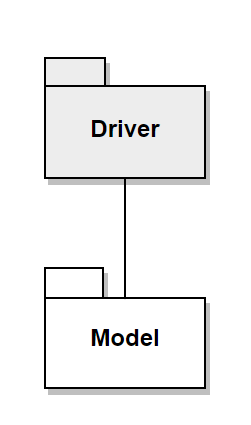
\includegraphics[width=0.2\linewidth]{Integration/I1.png}
        \label{fig:Integration_1}%
    \end{center}
\end{figure}


The integration of components will proceed with the Login and Registration features:

\begin{figure}[H]
    \begin{center}
        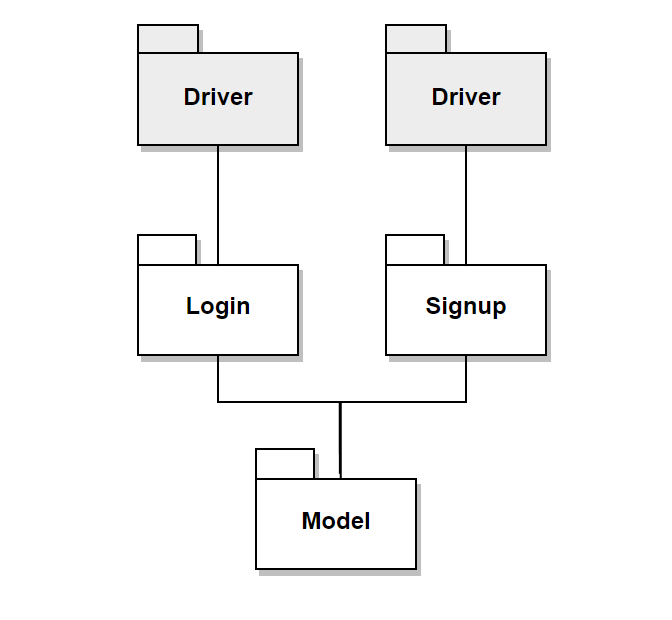
\includegraphics[width=0.4\linewidth]{Integration/I2.png}
        \label{fig:Integration_2}%
    \end{center}
\end{figure}

Once they will be developed and tested, it will be the turn of the components that perform a creation feature and their drivers:

\begin{figure}[H]
    \begin{center}
        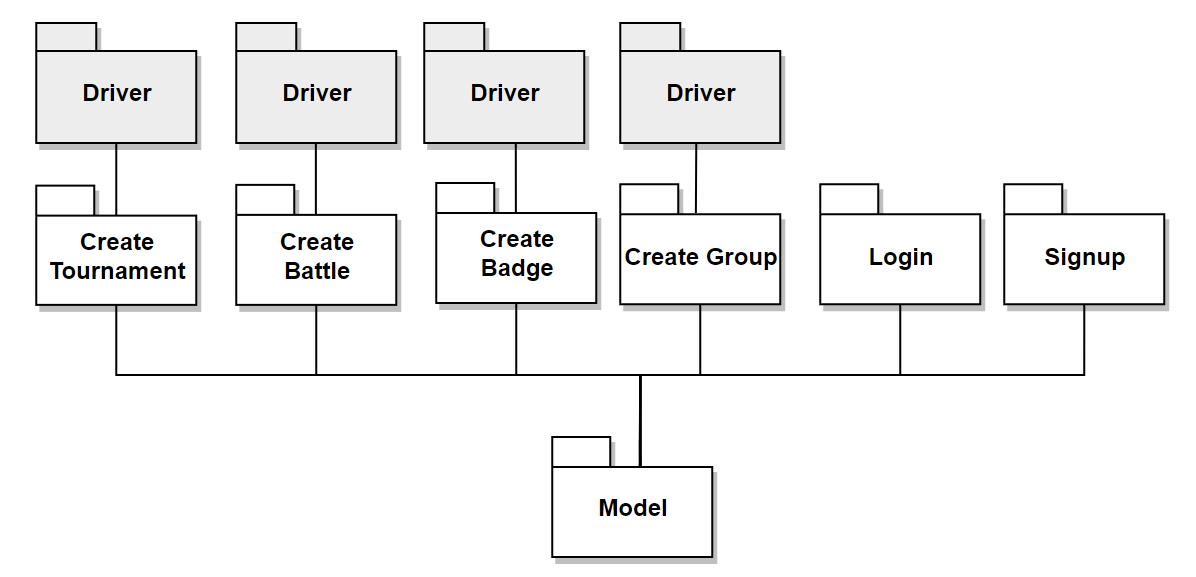
\includegraphics[width=0.8\linewidth]{Integration/I3.png}
        \label{fig:Integration_3}%
    \end{center}
\end{figure}

Now it is possible to create Tournaments, Battles, Groups and Badges functions to view those elements’ pages or the search components can be integrated.


\begin{figure}[H]
    \begin{center}
        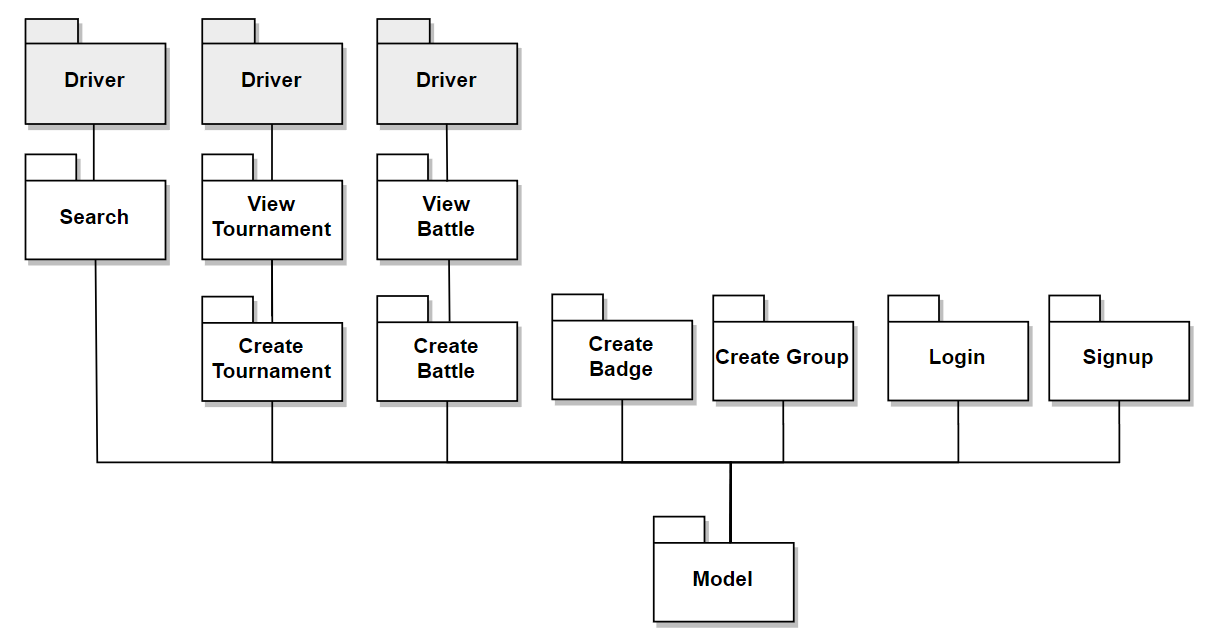
\includegraphics[width=0.8\linewidth]{Integration/I4.png}
        \label{fig:Integration_4}%
    \end{center}
\end{figure}

The last missing components in the context of Tournaments and Battles are the Join features, which will be integrated in parallel with the possibility to open Users’ profiles and to modify Badges parameters for the EDs.


\begin{figure}[H]
    \begin{center}
        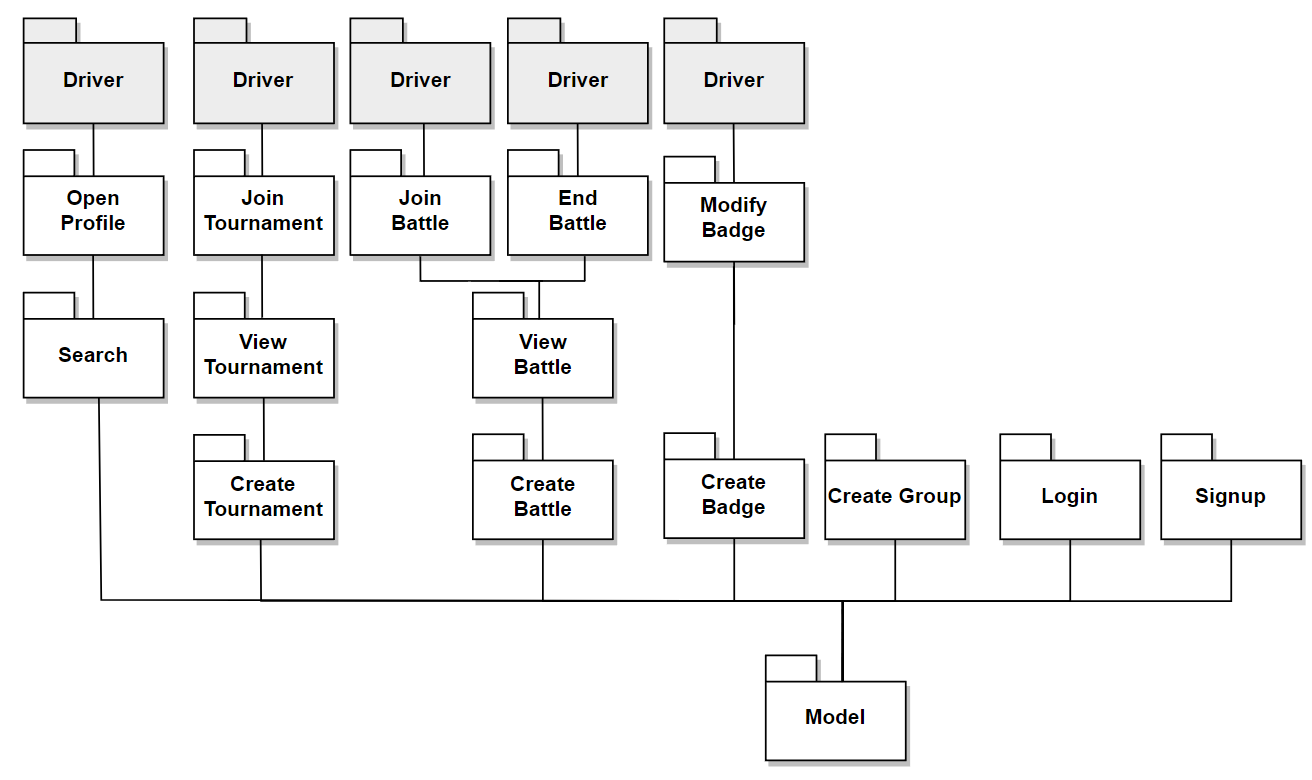
\includegraphics[width=0.8\linewidth]{Integration/I5.png}
        \label{fig:Integration_5}%
    \end{center}
\end{figure}

For the sake of simplicity, the previously integrated components are represented grouped in their Manager component (let the ‘Tournament Manager’ contain every Tournament-related component, and so on). Evaluation features will come next.

\begin{figure}[H]
    \begin{center}
        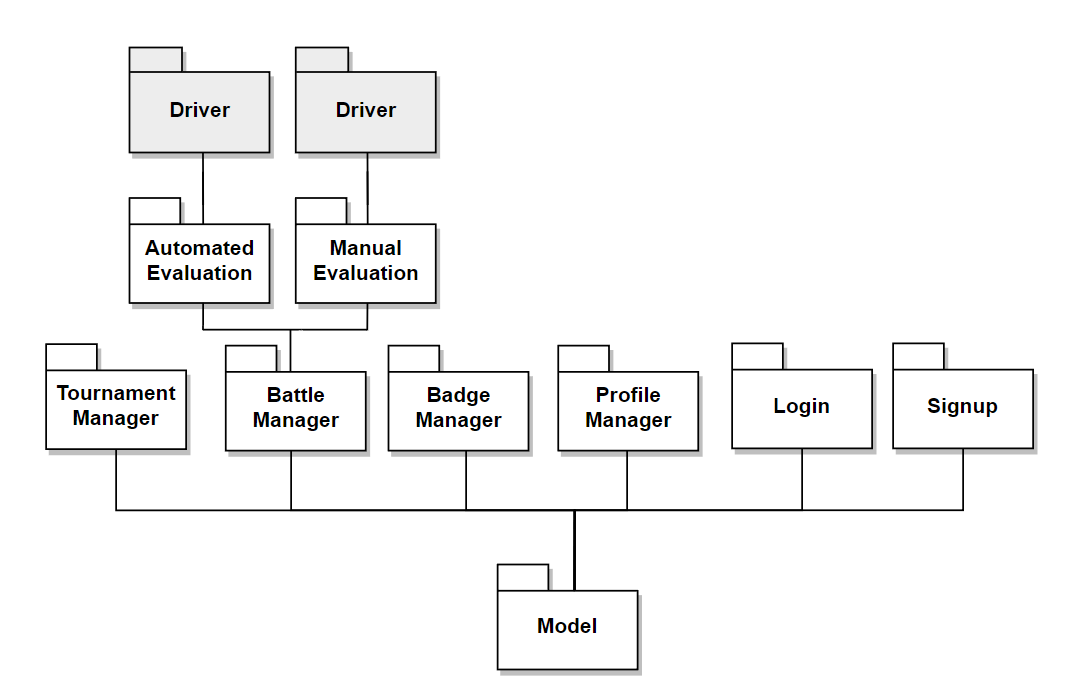
\includegraphics[width=0.8\linewidth]{Integration/I6.png}
        \label{fig:Integration_6}%
    \end{center}
\end{figure}

Once the Evaluation features are integrated, they will be considered as the same in the ‘Evaluation Manager’. Then Notification Manager will be the next to be integrated and tested.


\begin{figure}[H]
    \begin{center}
        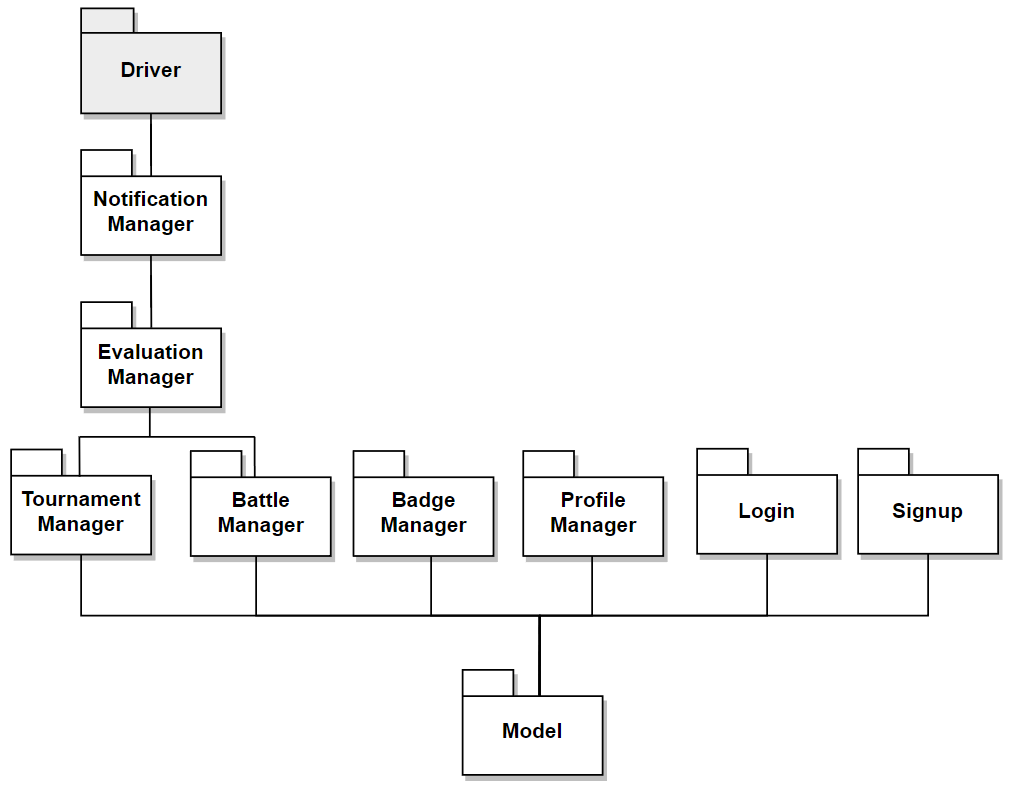
\includegraphics[width=0.8\linewidth]{Integration/I7.png}
        \label{fig:Integration_7}%
    \end{center}
\end{figure}

The last component that has to be integrated is the dashboard Manager, that is essential for the correct workflow of the user interface.


\begin{figure}[H]
    \begin{center}
        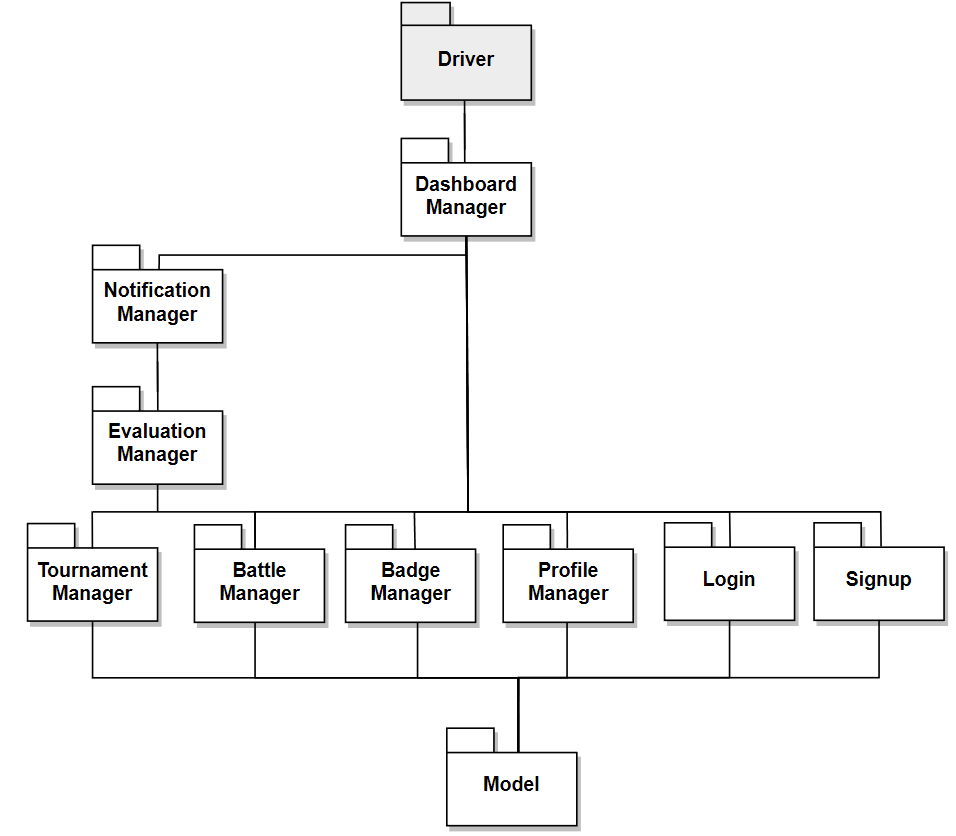
\includegraphics[width=0.8\linewidth]{Integration/I8.png}
        \label{fig:Integration_8}%
    \end{center}
\end{figure}

After the removal of the Dashboard Manager’s Driver, the final system is as follows.

\begin{figure}[H]
    \begin{center}
        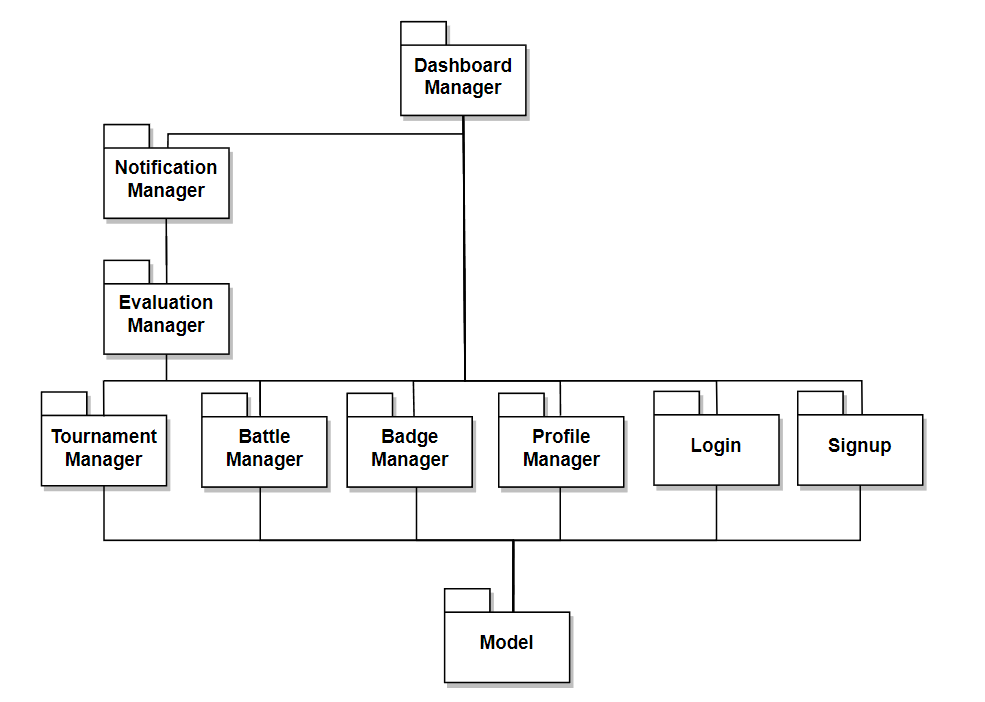
\includegraphics[width=0.8\linewidth]{Integration/IFinal.png}
        \label{fig:Integration_final}%
    \end{center}
\end{figure}



\section{System Testing Strategy}

It is necessary to check that each newly developed component works properly before integrating it with the system by the use of Drivers. Once a new component is integrated to the system, it must be checked with a new Driver that the new component is properly integrated, that the modules’ properties still hold and that the integrated system follows the correct workflow. 
Once every component is integrated, it will be needed to test the system as a whole to ensure the proper workflow is followed and the absence of bugs. In order to do so the following kinds of testing will be applied. 

\begin{itemize}
    \item \textbf{Functional Testing: }Functional Testing will be performed on the system to guarantee that the workflow is correct and consistent with the functionalities described in the RASD document, checking the fulfillment of goals, requirements and use cases and the possibility to correctly simulate the described scenarios. 
    \item \textbf{Load Testing:} Load Testing is useful in order to find eventual memory leaks, buffer overflows and bad management of memory.
    \item \textbf{Performance Testing:} The system will undergo this kind of testing in order to identify bottlenecks and to observe the resilience of the system under heavy workload, keeping in mind that the system shall support many users working simultaneously keeping response times as low as possible, following what is stated in the \textit{RASD document, section 3.3}. This will also help to identify optimization possibilities in the software’s algorithms.
    \item \textbf{Stress Testing:} In order to make sure that the system is capable of recovering itself after a failure, Stress Testing will be adopted, by simulating lots of concurrent users or reducing the system’s computational resources.
    \item \textbf{User Interface Testing:} It is important that the system correctly works on different kinds of devices, and different browsers as stated during the Requirements Analysis, testing the usability and accessibility of the web app on every possible platform, for both kinds of users: EDs and STs. 
\end{itemize}